%
% File: chap02.tex
% Author: Oliver J. H. Feighan
% Description: delta-scf benchmarking, including dft and dftb methods.
% Talk about important factors for modelling LHII
%
\let\textcircled=\pgftextcircled
\chapter{Mean-Field excited states}
\label{chap:dscf}

\initial {P}reamble

%=======
\section{Theory}
\label{sec:dscf_theory}

\subsection{$\Delta$-SCF and eigenvalue difference}
\label{subsec{dscf_and_eigdiff}}

\dscf predicts the excitation energy of a system by comparing the single point
energy of the ground state and the excited state. Finding this excited state
correctly can be an issue, but is usually assumed to be similar to the ground
state. In its simplest form, the \dscf method calculates the ground state, and
then calculates the excited state by rerunning an self-consistent field (SCF) 
with the excited state occupation numbers. This then gives a full description 
of both the ground as excited state from the orbital coefficients output from 
the two SCF procedures.

Initially, the excited state could be calculated by relaxing the orbitals which
contain the excited electron and hole in the ground state space, so that the
excited state and ground state are orthogonal\cite{Hunt1969}. However, it was
argued that this proceedure would exacerbate errors from finding the ground
state, and that the excited state was not a proper SCF solution\cite{Gilbert2008}.
Alternatively, it was proposed that an SCF like method, where instead of
populating orbitals according to the aufbau principle, orbitals which most
resemble the previous iteration's orbitals should be occupied. Each iteration 
in an SCF procedure produces new molecular orbital coefficients by solving the 
Roothaan-Hall equations\cite{Roothaan1951}, generally given as an eigenvalue problem:

\begin{equation}
\mathbf{F} \mathbf{C}^{\text{new}} = \mathbf{S} \mathbf{C}^{\text{new}} \epsilon
\end{equation}

where $\mathbf{C}^{\text{new}}$ are the next orbital coefficient solutions, 
$\mathbf{S}$ is the overlap, and $\epsilon$ are the orbital energies. 
The Fock matrix $\mathbf{F}$ is calculated from the previous set of orbital 
coefficients:

\begin{equation}
\mathbf{F} = f\left(\mathbf{C}^{\text{old}}\right)
\end{equation}

The amount of similarity of orbitals can be estimated from their overlap:

\begin{equation}
\mathbf{O} = \left(\mathbf{C}^{\text{old}}\right)^\dagger \mathbf{S} \mathbf{C}^{\text{new}}
\end{equation}

and for a single orbital can be evaluated as a projection:

\begin{equation}
p_j = \sum^n_i O_{ij} = \sum^N_\nu \left[\sum^N_\mu\left(\sum^n_i C_{i\mu}^{\text{old}}\right)S_{\mu\nu}\right]C^{\text{new}}_{\nu j}
\end{equation}

where $\mu,\nu$ are orbital indices. The population can then be given by the set
of orbitals with the highest projection $p_j$.  This method can be used for any
excited state, with the caveat that the orbital solution is in the same region
as the ground state solution. For a few low lying states, this is generally 
true, and so \dscf can be used to calculate a spectrum of excited states\cite{Gilbert2008}.
The method of using this orbital overlap is called the maximum overlap method (MOM).

\dscf has been shown to be cheap alternative to TDDFT and other higher level
methods, without considerable losses of accuracy in certain cases\cite{Worster2021}.
Additionally, as the excited state is given as solutions to SCF equations,
the gradient of this solution can be given by normal mean-field theory.
These gradients would be much cheaper than TDDFT or coupled cluster methods, and
so would be advantagous for a dynamic simulation of LHII.

The final descent in response theory would be to eigenvalue difference methods. 
Here there is assumed to be no response of the orbital energies and shapes when 
interacting with light. As stated earlier, this would be recovered from the
complete Cassida equation if the coupling elements in the $\mathbf{A}$ and 
$\mathbf{B}$ matrices are set to zero. This means that the difference between 
the excited state energy and the ground state energy is just the difference of
the orbital energies between the orbital an electron has been excited to and the
orbital has been excited from. Additionally, transition properties can be 
calculated by calculating transition density matrices from only the ground state.
Hence, all the information needed can be given by a single SCF optimization. 
Generally, eigenvalue difference methods are not seen as accurate response methods,
but can offer a quick and easy initial value\cite{Gimon2009}.

\subsection{Semi-empirical extensions}
\label{subsec:dscf_xtb}
We tried to extend the range of DFT methods that could be used for \dscf and 
eigenvalue difference methods by investigating whether a tight-binding method
could predict transition properties.
We chose the recently published DFTB method parameterized by the Grimme group for
this. This method has been parameterized for geometries, frequencies and non-covalent
interactions, and uses an extended version of H{\"u}ckel theory. The name they
present is GFN-xTB, standing for "Geometries, Frequencies, Non-Covalent - eXtended 
Tight Binding".
We chose this method for two reasons. The first being that the GFN-xTB method was
already implemented in the \code{QCORE} package. This significantly reduced the
amount of effort required for this project. Additionally, there would be other
users and developers who would help with implementation of this new method.
The second, more scientific reason, is that a similar method has already been
published that calculates transition properties. This is the sTDA-xTB method. 
As this method has similar goals as this project, it is useful to look at this 
in more detail.

\subsubsection{sTDA-xTB}
\label{subsubsec:stda_xtb}
A similar method to GFN1-xTB has already shown to be accurate at predicting
transition properties for large systems, with exceptional speed. This method was
published as the sTDA-xTB method\cite{Grimme2016}. The drop in accuracy for this
method is minimal, with the error being around 0.3 - 0.5 eV.

Similar to other xTB methods, the sTDA-xTB method is a tight-binding method that
uses empirically fit parameters and a minimal basis set. It was trained on a
test set of highly accurate coupled cluster and density functional theory
excitation energies, as well as accurate atomic partial charges.

Unlike other xTB methods, the basis set for sTDA-xTB is dependent on the D3
coordination number. This makes this method far more flexible, which would usually
be achieved in a fixed basis set by using diffuse or else additional orbitals in
the basis set. Additionally, it uses two sets of parameterized basis sets - a
smaller valence basis set (VBS) and an extended basis set (XBS).

These two basis sets are used to construct formally similar Fock matrix elements,
however in practice these use different global parameters. The core Hamiltonian
is similar to other DFTB methods that use a self-consistent charge method, as
opposed to an SCF method, to obtain molecular orbital coefficients. It is given by:

\begin{equation}
\bra{\psi_\mu} H^{\text{EHT, sTDA-xTB}} \ket{\psi_\mu}= \frac{1}{2} \left(k^l_\mu k^{l'}_\nu\right) \frac{1}{2} \left(h^l_\mu h^{l'}_\nu\right) S_{\mu\nu} - k_T \bra{\psi_\mu}\hat{T}\ket{\psi_\nu}
\end{equation}

where, $\mu,\nu,l,l'$ are orbital and shell indices  $k^l_\mu$ are shell-wise 
H{\"u}ckel parameters, $h$ are effective atomic-orbital energy levels, $S$ is
the overlap, $k_T$ is a global constant and $\hat{T}$ is the kinetic energy 
operator. The charges used in the inter-electronic repulsion function are given 
by CM5 charges for the XBS Fock matrix. These are calculated using Mulliken 
charges obtained from diagonalizng the Fock matrix with the VBS. The charges for 
the intial VBS Fock matrix are based on Gasteiger charges, modified by the 
electronegativities of atoms in the system.

The whole process for determining molecular orbitals can be summarized as:
\begin{enumerate}
	\item Calculate modifid Gasteiger charges for intial guess
	\item Diagonalize Fock matrix in the VBS to get the first set of Mulliken charges
	\item Compute CM5 charges
	\item Diagonalize Fock matrix in the VBS again for final set of Mulliken charges.
	\item Recalculate CM5 charges with this final set, and diagonalize the Fock matrix in the XBS. The molecular orbital coefficients from this are then fed to the response theory.
\end{enumerate}

The response theory for this method is based on the previous work in the Grimme 
group on the simplified Tann-Dancoff Approximation. There are several approximations 
made between full linear response theory and the sTDA method. First is the 
Tann-Danncoff approximation, where the B matrix is ignored. The second approximation 
is to use Mataga-Nishimoto-Ohno-Klopman (MNOK) integrals instead of explicit 2 electron 
integrals to calculate matrix elements, as well as neglecting the density 
functional term. 

Transition charges are used to calculate these MNOK integrals, where the charges 
are computed using a Löwdin population analysis. The operator is the 
MNOK\cite{Nishimoto1957}\cite{Ohno1964}\cite{Klopman1964} damped coloub function, 
with different exponents $y_K$ and $j_J$ for exchange and coulomb integral respectively. 
The $a_x$ parameter is included to recover the amount of Fock exchange mixing in
the original matrix element equation, and is a free parameter.

Third is the truncation of single particle excited space that is used to construct 
the $\mathbf{A}$ matrix. This reduces the number of elements that need to be 
calculated, and so reduces the time taken for diagonalization, whilst also capturing 
a broad enough spectrum of excitation energies. The sTDA-xTB has many of the same 
goals as this project, except in one respect, which is the gradient theory. As 
the sTDA-xTB method still requires constructing and diagonalizing the $\mathbf{A}$ 
matrix, albeit with a tight-binding method for molecular orbital coefficients, 
the gradient of the transition properties would still be difficult to calculate. 
Hence it wasn't used for this project, but informed us that an xTB like method 
could be used to get accurate transition properties.

\section{Benchmarking}
\label{sec:benchmarking}
Having established the hypothesis, that a GFN-xTB based \dscf method (which we
name \dxtb) would predict TD-DFT transition properties with decent accuracy, we
then tested this on a test set of small molecules, as well as bacterial chlorophylls
from the LHII protein. Additionally, we also investigated a \dscf with a DFT method
for the ground and excited state solutions, so we could compare the two differences
between the \dxtb method and our chosen reference method. The first being whether
the \dscf method can reproduce response effects, and the second being whether a
tight-binding, semi-empirical method could produce decent enough electronic
structure.

\subsection{Small Systems}
\label{subsec:smalltest}

\subsubsection{Non-orthogonality}
\label{subsubsec:dscf_nonorth}

\subsection{LHII Chlorophyll}
\label{subsec:dscf_chl_tests}

\subsection{GFN methods}
\label{subsec:dscf_gfn_tests}
We ran the same benchmarking set for the \dxtb method. Here we found it was 
necessary to extend the number methods that we were using to compare results.
Our range of methods were chosen to cover the different approximations for
transition properties we were making. Again the reference data was CC2 data, 
produced by the Grimme group. Our approximations were using \dscf rather than
linear response, and semi-empirical rather than DFT. Hence we investigated:
\begin{itemize}
    \item High level TD-DFT, with a range separated functional and large basis set
    \item Lower level TD-DFT, with a functional and smaller basis set
    \item \dscf with range separated functional and large basis set
    \item \dscf with functional and smaller basis set
    \item linear response with GFN-xTB
    \item \dscf with GFN-xTB, \dxtb
\end{itemize}

Concurrent to this work, we also implemented the GFN0-xTB method in \code{QCORE}.
This method is similar to the GFN-xTB method, but excludes any charge dependent
terms in its Fock matrix so is not self-consistent. We also tested whether this
would be a possibility for predicting transition properties.

The results are shown in fig.

\begin{figure}
    \includegraphics[]{../../Year_2/test_sets/sTDA_xtb_fit/stda_fit/HCNOF/dxtb_absolute_errors.png}
    \caption{A caption}
\end{figure}

\dxtb, in this initial form, as well as linear response GFN-xTB, is inaccurate 
at predicting excitation energies. The range of errors is quite large and there 
is a significant systematic shift in the errors as well. As the DFT methods, 
both the linear response and the \dscf methods, are quite accurate at predicting
the excitation energy, we conclude that the tight-binding method employed is the
leading cause of the error. 
There could be several factors for this error. For \dxtb, the excited state SCF 
cycle could converge to the wrong state or collapse to the ground state. This
would be evident by the symmetry of the excitation, as if the DFT and DFTB methods
converged to different states then the symmetry would also be different. We 
investigated how we might assign symmetries to \dxtb transitions, and \dscf in 
general. This is not a trivial task. 

\subsubsection{Post-SCF Assignment of Symmetry}
\label{subsubsec:post_scf_symmetry}

Considering symmetry is a common thread in many parts of electronic structure 
theory. It appears in normal mode analysis, wavefunction analysis and assignment
of electronic transitions. For this project, we looked at assigning symmetry to 
the transitions for \dscf methods, which would require assigning symmetry to the
orbitals and overall wavefunction of a molecule.
Broadly speaking, most electronic structure codes have two choices in assigning
symmetry to orbitals - either all of the SCF code will treat symmetry from the 
outset, or nothing is assigned in the SCF code and assignment will happen post-SCF.
Both these approaches have benefits and drawbacks. The first method allows the 
symmetry to be given at any point in the SCF procedure, so allows the Hamiltonian
to be organized into a block diagonal matrix, which can be useful when solving
for a large basis set or large system. However, this is only true if the system 
is highly symmetric, which is often not the case when treating systems from a 
molecular dynamics simulation, and definitely not the case when looking at biological
systems.
The second approach doesn't fix these drawbacks, but it does allow for codes which
originally didn't have symmetry assignment to be extended without rewriting SCF
code. The obvious drawback of doing assignment post-SCF is that symmetry can't be
utilized during the SCF procedure.
We opted for the second approach, as this was the easiest to implement. We used 
the open source library libmsym for point group assignment routines and finding
the symmetry adapted linear combination of atomic orbitals. Broadly, the outline
of assigning orbital symmetry is as follows:
\begin{enumerate}
    \item Determine the point group of the molecule, from the atomic positions
    \item Setup the atomic orbitals in the libmsym representation.
    \item Get the symmetry adapted linear combination (SALC) of atomic orbitals for 
    each subspace. These subspaces are the groups of symmetries that can be found
    in the point group of the molecule.
    \item The SALC can then be used to make the transformation matrix $T$.
    \item Assign the one electron molecular orbital (MO) for these subspace characters
     with the symmetry adapted linear combinations.
    \item Multiply the one electron MO symmetries together to find the symmetry 
    of the overall wavefunction.
\end{enumerate}

\begin{figure}
    \centering
    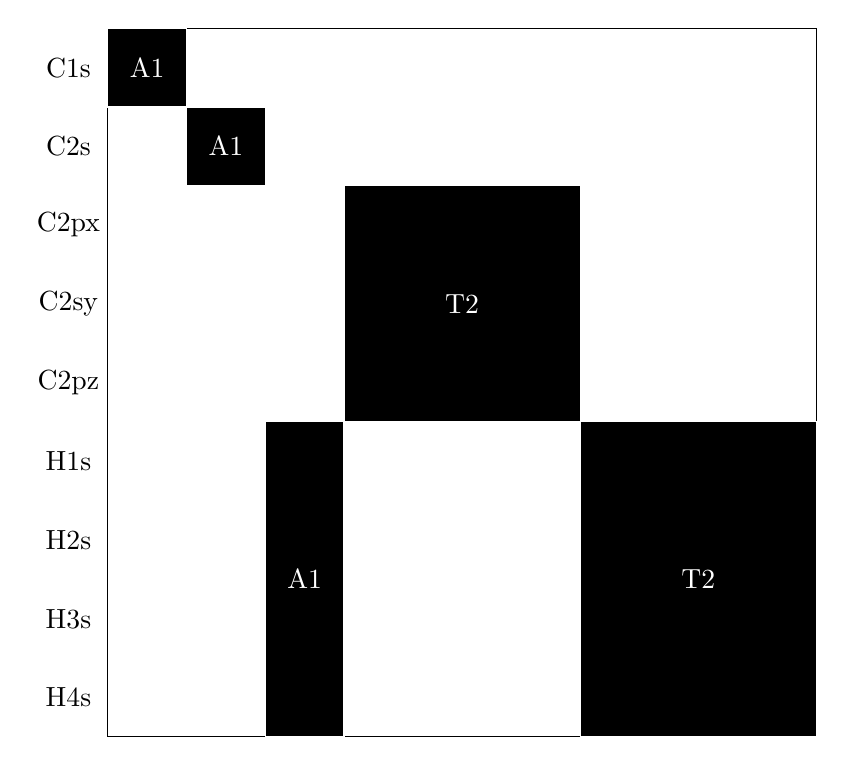
\begin{tikzpicture}
        \node[draw=none,
        rectangle, 
        minimum width = 1cm, 
        minimum height = 1cm
        ](r) at (-5cm,4cm) {C1s};
        \node[draw=none,
        rectangle, 
        minimum width = 1cm, 
        minimum height = 1cm
        ](r) at (-5cm,3cm) {C2s};
        \node[draw=none,
        rectangle, 
        minimum width = 1cm, 
        minimum height = 1cm
        ](r) at (-5cm,2cm) {C2px};
        \node[draw=none,
        rectangle, 
        minimum width = 1cm, 
        minimum height = 1cm
        ](r) at (-5cm,1cm) {C2sy};
        \node[draw=none,
        rectangle, 
        minimum width = 1cm, 
        minimum height = 1cm
        ](r) at (-5cm,0cm) {C2pz};
        \node[draw=none,
        rectangle, 
        minimum width = 1cm, 
        minimum height = 1cm
        ](r) at (-5cm,-1cm) {H1s};
        \node[draw=none,
        rectangle, 
        minimum width = 1cm, 
        minimum height = 1cm
        ](r) at (-5cm,-2cm) {H2s};
        \node[draw=none,
        rectangle, 
        minimum width = 1cm, 
        minimum height = 1cm
        ](r) at (-5cm,-3cm) {H3s};
        \node[draw=none,
        rectangle, 
        minimum width = 1cm, 
        minimum height = 1cm
        ](r) at (-5cm,-4cm) {H4s};
        
        \node[draw,
        rectangle, 
        minimum width = 9cm, 
        minimum height = 9cm
        ](r) at (0cm,0cm) {};

        \node[draw,
        rectangle, 
        color=white,
        fill=black,
        minimum width = 1cm, 
        minimum height = 1cm
        ](r) at (-4cm,4cm) {A1};

        \node[draw,
        rectangle,
        color=white, 
        fill=black,
        minimum width = 1cm, 
        minimum height = 1cm
        ](r) at (-3cm,3cm) {A1};

        \node[draw,
        rectangle,
        color=white,
        fill=black,
        minimum width = 1cm, 
        minimum height = 4cm
        ](r) at (-2cm,-2.5cm) {A1};

        \node[draw,
        rectangle, 
        color=white,
        fill=black,
        minimum width = 3cm, 
        minimum height = 3cm
        ](r) at (0cm,1cm) {T2};

        \node[draw,
        rectangle, 
        color=white,
        fill=black,
        minimum width = 3cm, 
        minimum height = 4cm
        ](r) at (3cm,-2.5cm) {T2};

    \end{tikzpicture}
    \caption{Symmetry assigned MOs}
\end{figure}


We implemented this procedure and tested this on methane with a minimal basis set.
We found that we could accurately assign the MOs and overall wavefunction of this
system with this method for the ground state, which was encouraging.
However, we encountered two problems. First was that the assignment of MOs broke
down for excited states. The second was that for non-abelian groups, where there
are some degenerate subspaces such as E and T, this assignment also didn't work.
We discussed some ideas about using symmetry decomposition for the non-abelian 
point groups, but as this was a short study we decided that this might not be the
most prudent path. Hence, we could not confidently assign transitions from \dscf
methods with this method. The importance of this is that symmetry couldn't be 
assigned automatically. We still had the method of assigning transitions by looking
at transition dipoles and plots of molecular orbitals, but these methods require
a person to look at the problem at hand. This makes any benchmarking a lengthy 
process, which isn't repeatable as we extend the methods included in the benchmarking.

\subsubsection{Implications of Benchmarking Results}
\label{subsubsec:imp_of_benchmarking}
There may also be inaccurate treatment of inter-electronic repulsion and correlation 
which is found in other tight binding methods. Additionally, the parameters in 
GFN1 and GFN0 are not optimized for excited states.

We also investigated an eigenvalue difference method, using eigenvalues from the
\code{xtb4stda} program. This is the program that provides the molecular orbital
coefficients for the \code{stda} program. This was done to initially 
investigate whether an eigenvalue difference method for a excited state parameterized 
method would be accurate, but this proves to not be the case.

\section{Extensibility}
\label{sec:dscf_problems}

\subsection{Embedding}
\label{subsec:dscf_embedding}

\subsection{Scaling}
\label{subsec:dscf_scaling}